\documentclass[a4paper,11pt]{article}

\usepackage[utf8]{inputenc}
\usepackage[swedish]{babel}
\usepackage[top=1in,bottom=1in,left=1in,right=1in,headsep=.5in]{geometry}
\usepackage{hyperref}
\usepackage{graphicx}

\usepackage{array}
\newcolumntype{L}[1]{>{\raggedright\let\newline\\\arraybackslash\hspace{0pt}}m{#1}}
\newcolumntype{C}[1]{>{\centering\let\newline\\\arraybackslash\hspace{0pt}}m{#1}}
\newcolumntype{R}[1]{>{\raggedleft\let\newline\\\arraybackslash\hspace{0pt}}m{#1}}

\usepackage[yyyymmdd,hhmmss]{datetime}
\renewcommand{\dateseparator}{-}

\usepackage{mathptmx}    %Times Roman font
\usepackage{helvet}    %Helvetica, served as a model for arial
\usepackage{anyfontsize}

\usepackage[tocgraduated]{tocstyle}
\usetocstyle{allwithdot}

\usepackage[titletoc,title]{appendix}

\usepackage{fancyhdr}
\fancypagestyle{intro}{
    \fancyhf{}
    \fancyhead[C]{\LIPSprojekttitel}
    \fancyhead[R]{\today} 
    \fancyfoot[L]{\LIPSkursnamn \\ \LIPSdokumenttyp}
    \fancyfoot[C]{\phantom{text}\roman{page}}
    \fancyfoot[R]{\LIPSprojektgrupp \\ \LIPSgruppepost} 
    \renewcommand{\headrulewidth}{0.4pt}
    \renewcommand{\footrulewidth}{0.4pt}}
\fancypagestyle{content}{
    \fancyhf{}
    \fancyhead[C]{\LIPSprojekttitel}
    \fancyhead[R]{\today} 
    \fancyfoot[L]{\LIPSkursnamn \\ \LIPSdokumenttyp}
    \fancyfoot[C]{\phantom{text}\thepage}
    \fancyfoot[R]{\LIPSprojektgrupp \\ \LIPSgruppepost} 
    \renewcommand{\headrulewidth}{0.4pt}
    \renewcommand{\footrulewidth}{0.4pt}}

\usepackage{titlesec}
\titleformat{\section}
    {\normalfont\sffamily\Large\bfseries}
    {\thesection}{1em}{}
\titleformat{\subsection}
    {\normalfont\sffamily\large\bfseries}
    {\thesubsection}{1em}{}
\titleformat{\subsubsection}
    {\normalfont\sffamily\bfseries}
    {\thesubsubsection}{1em}{}

\newcommand{\LIPSartaltermin}{2016/HT}
\newcommand{\LIPSkursnamn}{TSEA29}
\newcommand{\LIPSprojekttitel}{Kartrobot}
\newcommand{\LIPSprojektgrupp}{Grupp 1}
\newcommand{\LIPSgruppepost}{\href{mailto:kmm_2016_grupp1@liuonline.onmicrosoft.com}{{\small kmm\_2016\_grupp1@liuonline.onmicrosoft.com}}}
\newcommand{\LIPSgrupphemsida}{}
\newcommand{\LIPSkund}{ISY, Linköpings universitet, 581\,83 Linköping}
\newcommand{\LIPSkundkontakt}{Mattias Krysander, 013-282198, matkr@isy.liu.se}
\newcommand{\LIPSkursansvarig}{Tomas Svensson, 013-281368, Tomas.Svensson@liu.se}
\newcommand{\LIPShandledare}{}
\newcommand{\LIPSdokumenttyp}{Systemskiss}
\newcommand{\LIPSredaktor}{Hannes Haglund}
\newcommand{\LIPSversion}{0.1}
\newcommand{\LIPSgranskare}{Felix Härnström}
\newcommand{\LIPSgranskatdatum}{N/A}
\newcommand{\LIPSgodkannare}{}
\newcommand{\LIPSgodkantdatum}{}

\newcommand{\LIPStitelsida}{
\vspace*{200pt}
\renewcommand{\familydefault}{\sfdefault}	%Sans-serif
\normalfont
\begin{center}
{\fontsize{18}{22}\selectfont \textbf{\MakeUppercase{\LIPSdokumenttyp}}}
\end{center}
\begin{center}
{\fontsize{12}{14}\selectfont \LIPSredaktor \\[8pt] Version \LIPSversion}
\end{center}
\vspace*{220pt}
\begin{center}
{\fontsize{12}{14}\selectfont Status}
\end{center}
\begin{center}
\setlength\extrarowheight{2pt}
\begin{tabular}{| L{100pt} | L{100pt} | L{100pt} |}
\hline 
Granskad & \LIPSgranskare & \LIPSgranskatdatum \\
\hline 
Godkänd & \LIPSgodkannare & \LIPSgodkantdatum \\ 
\hline 
\end{tabular} 
\end{center}
\renewcommand{\familydefault}{\rmdefault}	%Back to serifs
\normalfont
}


\newenvironment{LIPSprojektidentitet}{%
\vspace*{200pt}
\renewcommand{\familydefault}{\sfdefault}	%Sans-serif
\normalfont
\begin{center}
{\fontsize{16}{19}\selectfont \textbf{PROJEKTIDENTITET}}
\end{center}
\renewcommand{\familydefault}{\rmdefault}	%Back to serifs
\normalfont
\begin{center}
\LIPSartaltermin, \LIPSprojektgrupp \\ Linköpings tekniska högskola, ISY
\end{center}
\renewcommand{\familydefault}{\sfdefault}	%Sans-serif
\normalfont
\vspace*{10pt}
\begin{center}
\setlength\extrarowheight{2pt}
\begin{tabular}{| L{100pt} | L{150pt} | L{150pt} |}
\hline
\textbf{Namn} & \textbf{Ansvar} & \textbf{E-post} \\
}%
{%
\hline
\end{tabular} 
\end{center}
\renewcommand{\familydefault}{\rmdefault}	%Back to serifs
\normalfont
\begin{center}
\textbf{E-postlista för hela gruppen:} \LIPSgruppepost \\
\textbf{Hemsida:} \LIPSgrupphemsida \\
\vspace*{15pt}
\textbf{Kund:} \LIPSkund \\
\textbf{Kontaktperson hos kund:} \LIPSkundkontakt \\
\vspace*{15pt}
\textbf{Kursansvarig:} \LIPSkursansvarig \\
\textbf{Handledare:} \LIPShandledare \\
\end{center}
}
\newcommand{\LIPSgruppmedlem}[3]{\hline {#1} & {#2} & \href{mailto:{#3}}{{#3}} \\}

\newenvironment{LIPSdokumenthistorik}{%
\vspace*{100pt}
\renewcommand{\familydefault}{\sfdefault}	%Sans-serif
\normalfont
\begin{center}
{\fontsize{14}{17}\selectfont \textbf{Dokumenthistorik}}
\end{center}
\begin{center}
\setlength\extrarowheight{2pt}
\begin{tabular}{| L{50pt} | L{60pt} | L{150pt} | L{60pt} | L{55pt} |}
\hline
\textbf{Version} & \textbf{Datum} & \textbf{Utförda förändringar} & \textbf{Utförda av} & \textbf{Granskad} \\
}%
{%
\hline
\end{tabular} 
\end{center}
\renewcommand{\familydefault}{\rmdefault}	%Back to serifs
\normalfont
}
\newcommand{\LIPSversionsinfo}[5]{\hline {#1} & {#2} & {#3} & {#4} & {#5} \\}

\newcounter{LIPSkravnummer}
\newcounter{LIPSunderkravnummer}[LIPSkravnummer]
\newenvironment{LIPSkravlista}{%
\renewcommand{\familydefault}{\sfdefault}	%Sans-serif
\normalfont
 \setlength\extrarowheight{2pt}
  \begin{tabular}{| L{30pt } | L{60pt} | L{250pt} | L{50pt} |}
    }%
  {%
    \hline
  \end{tabular}
\renewcommand{\familydefault}{\rmdefault}	%Back to serifs
\normalfont
}
\newcommand{\LIPSkrav}[3]{\hline\stepcounter{LIPSkravnummer}\textbf{\arabic{LIPSkravnummer}} & \textbf{{#1}} & {#2} & \textbf{{#3}} \\}

\newcommand{\LIPSkravDemo}[3]{\hline\textbf{X} & \textbf{{#1}} & {#2} & \textbf{{#3}} \\}

\newcommand{\LIPSunderkrav}[3]{\hline\stepcounter{LIPSunderkravnummer}\textbf{\arabic{LIPSkravnummer}\Alph{LIPSunderkravnummer}} & \textbf{{#1}} & {#2} & \textbf{{#3}} \\}


\newenvironment{LIPSleveranslista}{
\renewcommand{\familydefault}{\sfdefault}	%Sans-serif
\normalfont
	\setlength\extrarowheight{2pt}
	\begin{tabular}{| L{25mm} | L{25mm} | L{55mm} | L{25mm} | L{5mm} |} 
	}
	{
		\hline
	\end{tabular}
\renewcommand{\familydefault}{\rmdefault}	%Back to serifs
\normalfont
}
\newcommand{\LIPSleverans}[4]{ \hline\stepcounter{LIPSkravnummer}\textbf{Krav nr \arabic{LIPSkravnummer}}&\textbf{{#1}}&{#2}&\textbf{{#3}}&\textbf{{#4}}\\}


\newenvironment{LIPSdokumentlista}{%
	\renewcommand{\familydefault}{\sfdefault}	%Sans-serif
	\normalfont
	\setlength\extrarowheight{2pt}
	\begin{tabular}{| L{40mm} | L{13mm} | L{50mm} | L{19mm} | L{14mm} |} 
		
		\hline
		\textbf{Dokument} & \textbf{Språk} & \textbf{Syfte/Innehåll} & \textbf{Målgrupp} & \textbf{Format} \\
	}%
	{%
		\hline
	\end{tabular}
	\renewcommand{\familydefault}{\rmdefault}	%Back to serifs
	\normalfont
}
\newcommand{\LIPSdokument}[5]{\hline {#1} & {#2} & {#3} & {#4} & {#5}\\}

\begin{document}
\pagestyle{intro}
\LIPStitelsida
\clearpage
\begin{LIPSprojektidentitet}
    \LIPSgruppmedlem{Hannes Haglund}{}{hanha265@student.liu.se}
    \LIPSgruppmedlem{Felix Härnström}{Projektledare (PL)}{felha423@student.liu.se}
    \LIPSgruppmedlem{Jani Jokinen}{}{janjo273@student.liu.se}
    \LIPSgruppmedlem{Silas Lenz}{}{sille914@student.liu.se}
    \LIPSgruppmedlem{Daniel Månsson}{}{danma344@student.liu.se}
    \LIPSgruppmedlem{Emil Norberg}{Dokumentansvarig (DOK)}{emino969@student.liu.se}
\end{LIPSprojektidentitet}
\clearpage
\renewcommand{\familydefault}{\sfdefault}	%Sans-serif
\normalfont
\tableofcontents
\renewcommand{\familydefault}{\rmdefault}	%Back to serifs
\normalfont
\clearpage
\begin{LIPSdokumenthistorik}
    \LIPSversionsinfo{0.1}{1496-05-12}{Första utkastet}{Alla}{N/A} %TODO granskare
\end{LIPSdokumenthistorik}
\clearpage
\setcounter{page}{1}
\pagestyle{content}

\section{Inledning}

I detta dokument redogörs idéer om hur robotens delsystem kan konstrueras. Det är ej bindande, utan tjänar snarare som en grov kompass inför projektets implementation och planering. Skissen används för att avgöra vilka moduler som ingår och hur arbetet kan delas upp.

\begin{figure}[h!]
    \makebox[\textwidth][c]{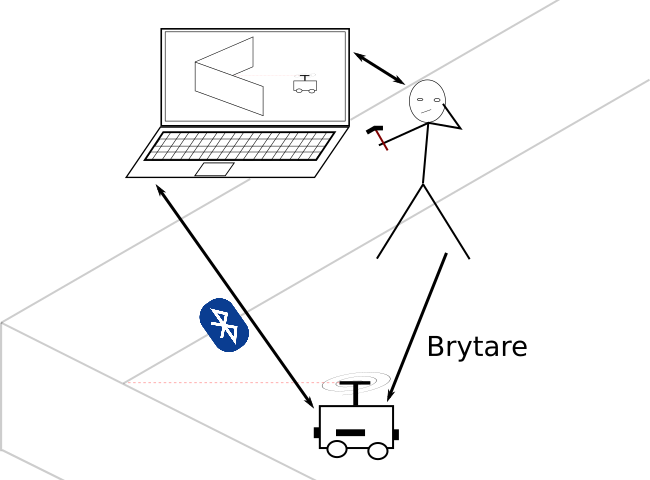
\includegraphics[width=1\textwidth]{overview.png}}
    \caption{Systemet i dess omgivning.}
    \label{fig:overview}
\end{figure}

\section{Översikt av systemet}
% TODO: Blockschema, identifiera delsystem och gränssnitt, modularitet och uppgraderbarhet


\section{Delsystem 1 - Sensorenhet}

Sensorenheten har i uppgift att läsa in sensordata och omvandla den till ett läsligt format.


\subsection{Hårdvara}

Sensorenheten tar in data från en distanssensor monterade på robotens topp.
\subsubsection{Processor} %TODO: Minst 4 interrupts, fråga handledare. Kan vi ha flera uarts?
% Troligtvis Atmega1284p
\subsubsection{Ultraljudssensor} \label{sssec:sonicsensors}

% TODO: Alt 2 IRSensor

\subsubsection{LIDAR lite v2} \label{sssec:lidar}
LIDAR är en kraftfull lasersensor som i systemet som helhet används för mätningar som kräver en viss grad av noggranhet. Komponenten kan kommuniceras med via en I\textsuperscript{2}C-buss, som därmed ska användas, se sektion \ref{ssec:sensorInterface}. Processorn behöver mjukvarustöd för detta.

Sensorn monteras på toppen av roboten - ovanpå en roterande servo, som specificeras i större detalj i sektion \ref{ssec:servomotor}. Detta för att effektivt kunna mäta avstånd i flera vinklar.

\subsubsection{IMU} \label{sssec:imu}

\paragraph{Alternativ 1}
Endast en gyro med analog output.

\paragraph{Alternativ 2}
Gyro+Accelerometer via I\textsuperscript{2}C. mpu6050 % TODO: MotionMagi, handledare

\subsection{Mjukvara}

Koden ska vara skriven i C, och ska följa <INSERT STANDARD HERE>. Funktioner ska vara kommenterade.

Programmet ska omvandla sensordata till ett mer läsligt format, och ska kunna skicka det vidare (se \ref{ssec:sensorInterface}).

\subsection{Gränssnitt} \label{ssec:sensorInterface}
Sensorenheten kommer behöva kommunicera med de faktiska sensorerna, samt ha ett sätt att passera vidare utdata. Sensorenheten tar inte emot någon indata, och kan inte styras.
%TODO more detailed explenation in general? Specifications around i2c and sonic-sensors output and stuff.
% TODO: A nice picture featuring hardware and interfaces

\subsubsection{LIDAR och gyro}
Då LIDAR lite v2 (\ref{sssec:lidar}) och gyron (\ref{sssec:imu}) kräver en I\textsuperscript{2}C-buss så kommer en sådan att användas för kommunikation mellan dem och processorn. Vi supportar inte flera masters, utan behandlar processorn som den enda, med LIDAR:n och gyron som slavar.

\subsubsection{Ultraljudssensorer}
Ultraljudssensorerna (\ref{sssec:sonicsensors}) är betydligt mer lågnivå i sina gränssnitt, och kommunicerar via spänningsskillnader. Deras utvärde beror på längden på dess höga signal, så för att garantera att vi börjar mäta omedelbart på en hög flank så ska avbrott utnyttjas. Detta uppnås genom att helt enkelt daisy-chaina denna signal till en av avbrottsportarna på processorns

\subsubsection{Utvärden}
Hur passeras processerade mätvärden vidare?

\paragraph{Alternativ 1}
I\textsuperscript{2}C-bussen som användes för att kommunicera med LIDAR:n och gyron kan utnyttjas, med även processorn som slav. Enheten som tar emot data från sensorenheten får istället ta över den rollen.

\paragraph{Alternativ 2}
Att skicka utdata via UART är en relativt enkel och elegant lösning.

\subsubsection{IN}

\subsubsection{UT}



\section{Delsystem 2 - Styrenhet}

\subsection{Hårdvara}

\subsubsection{Processor}
%Samma som sensorenhet

\subsubsection{PWM-utgångar}

\subsubsection{Servo/steppermotor} \label{ssec:servomotor}
\paragraph{Alternativ 1}
AX-12

\subsection{Mjukvara}

Koden ska vara skriven i C, och ska följa <INSERT STANDARD HERE>. Funktioner ska vara kommenterade.

\subsection{Gränssnitt} \label{ssec:controllInterface}

\subsubsection{Alternativ 1}

\subsubsection{Alternativ 2}


\section{Delsystem 3 - Kommunikations- och kontrollenhet}

\subsection{Hårdvara}

\subsubsection{Datormodell}
Raspberry Pi 3. Vi utnyttjar raspberryns inbyggda blåtand.

\subsection{Mjukvara}

Koden ska vara skriven i Python 3, och ska följa kodstandarden \href{https://www.python.org/dev/peps/pep-0008/}{PEP 8}.

\subsubsection{Kommunikation}

\subsubsection{Ruttstyrning}

\subsection{Gränssnitt} \label{ssec:brainInterface}

\subsubsection{Alternativ 1}
I\textsuperscript{2}C via samma buss som sensorer

\subsubsection{Alternativ 2}
USB-UART

\section{Delsystem 4 - Mjukvara på PC}

\subsection{Hårdvara}
Har en blåtandsmodul.

\subsection{Mjukvara}

Koden ska vara skriven i Python 3, och ska följa kodstandarden \href{https://www.python.org/dev/peps/pep-0008/}{PEP 8}.

\subsubsection{Input}

\subsubsection{Output}

\subsection{Gränssnitt} \label{ssec:PCInterface}


\begin{appendices}

\end{appendices}


\end{document}
